% Fase 3B, exemplos 11–12. Fontes: mb-uso/secoes.
\begin{frame}[fragile]{Exemplo 11 — Por que referências diferentes podem inverter o HV?}
\textbf{DTLZ2, NSGA-II, 50 gerações, cinco repetições:} comparar populações de 20 e 100 indivíduos.
\begin{columns}[T,onlytextwidth]
\begin{column}{.48\textwidth}
\begin{lstlisting}[style=python,basicstyle=\ttfamily\fontsize{7.3}{9.1}\selectfont]
# exp1: 20 individuos
# exp2: 100 individuos
h1 = mb.metrics.hv(exp1, scale='raw')
h2 = mb.metrics.hv(exp2, scale='raw')
print(h1.last, h2.last)
\end{lstlisting}
\textbf{Referências individuais:}
\par Pop. 20: \textbf{0,959673}
\par Pop. 100: \textbf{0,843102}
\par\smallskip
Nesse cálculo, a população de 20 parece superior, mas as réguas de normalização são distintas.
\end{column}
\begin{column}{.50\textwidth}
\centering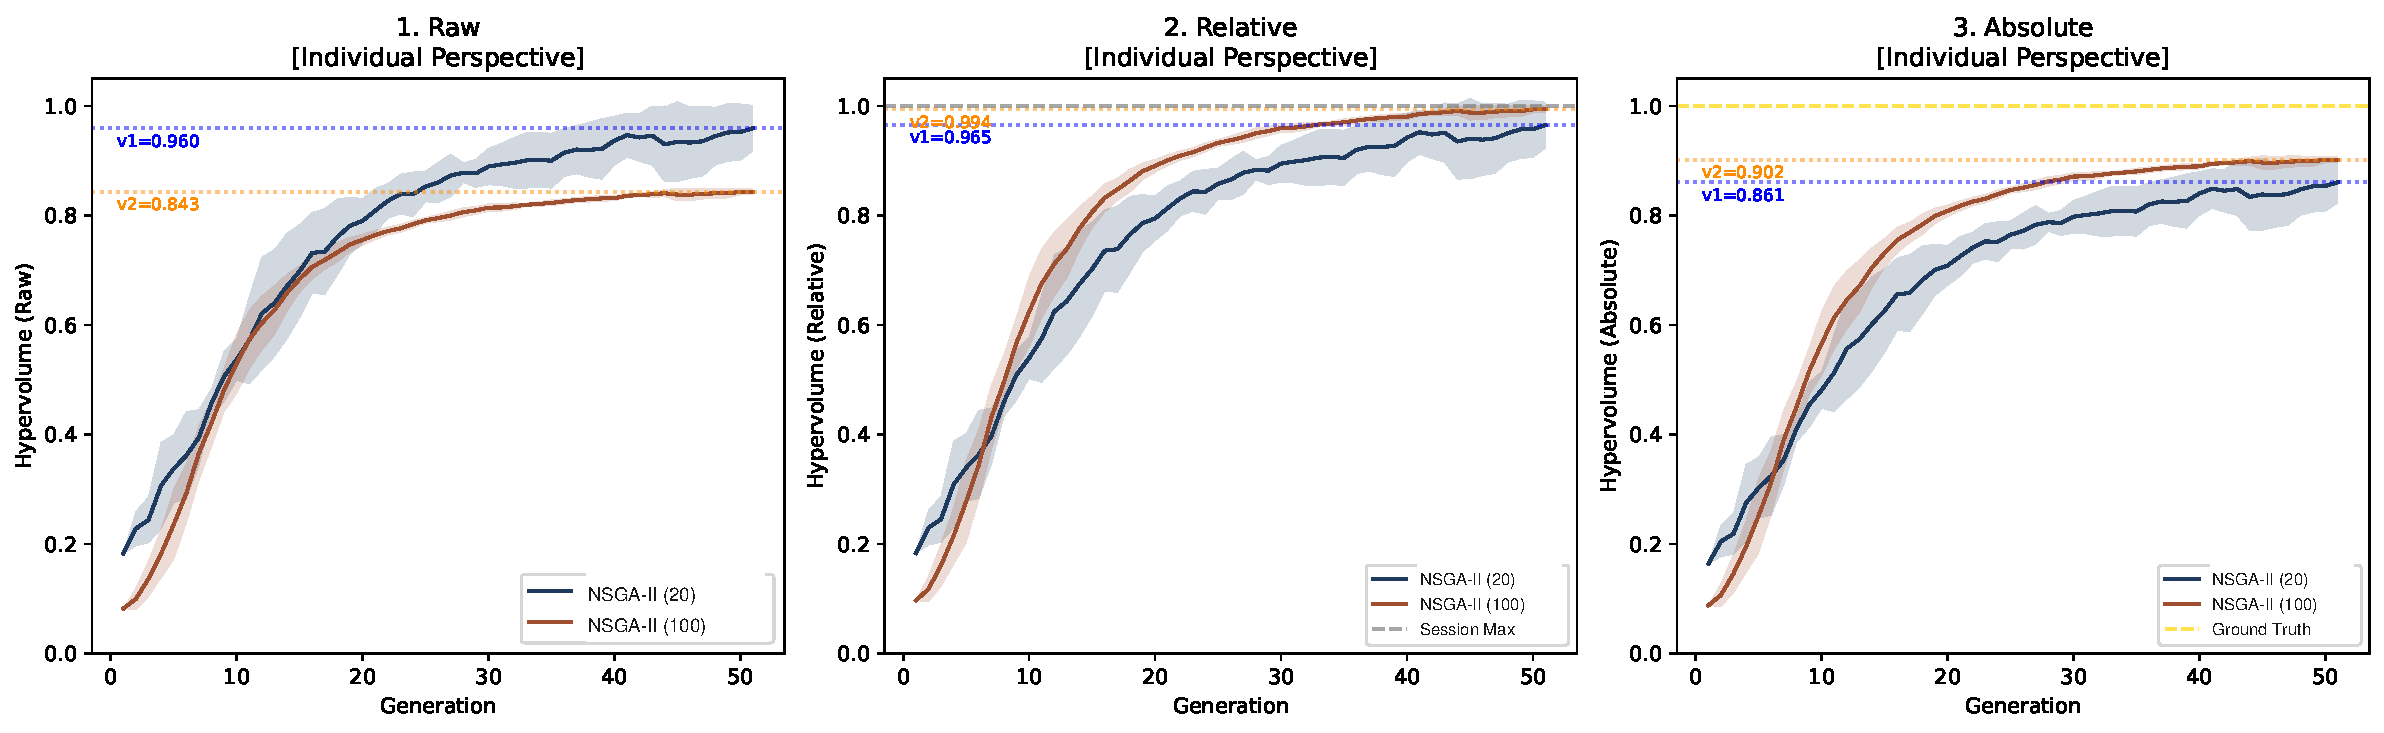
\includegraphics[width=\linewidth,height=.57\textheight,keepaspectratio]{figures/example_15_composite_01.pdf}
\par{\scriptsize Históricos para HV bruto, relativo e absoluto com referências individuais.}
\end{column}
\end{columns}
\end{frame}

\begin{frame}[fragile]{Exemplo 11 — A referência compartilhada altera a conclusão}
\begin{columns}[T,onlytextwidth]
\begin{column}{.57\textwidth}
\centering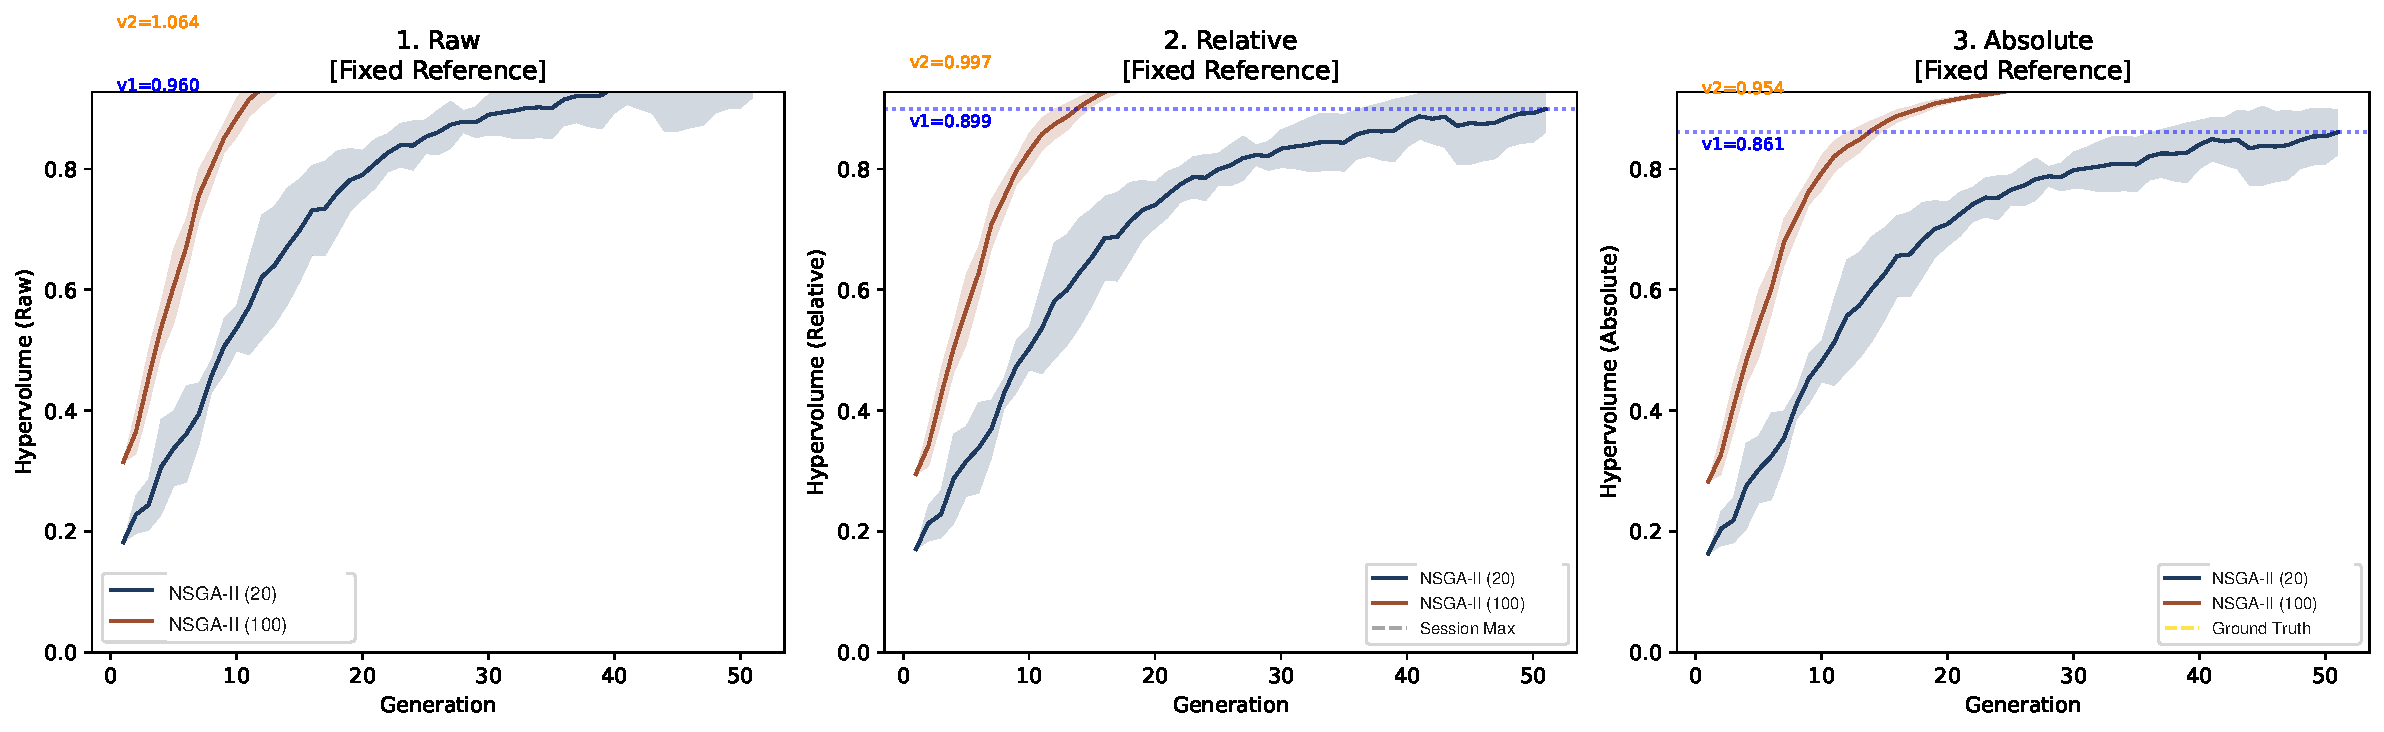
\includegraphics[width=\linewidth,height=.57\textheight,keepaspectratio]{figures/example_15_composite_02.pdf}
\end{column}
\begin{column}{.41\textwidth}
\begin{lstlisting}[style=python,basicstyle=\ttfamily\fontsize{7.2}{8.9}\selectfont]
ref = [exp1, exp2]
h1c = mb.metrics.hv(
    exp1, ref=ref, scale='raw')
h2c = mb.metrics.hv(
    exp2, ref=ref, scale='raw')
print(h1c.last, h2c.last)
\end{lstlisting}
\textbf{HV bruto comum:}
\par Pop. 20: \textbf{0,959673}
\par Pop. 100: \textbf{1,063889}
\end{column}
\end{columns}
\vspace{.05cm}\textbf{A ordenação se inverte:} a população de 100 passa a ter melhor HV. O experimento não mudou: mudou a régua. Na comparação de algoritmos, é indispensável explicitar uma referência compartilhada.
\end{frame}

\begin{frame}[fragile]{Exemplo 12 — Variabilidade espacial em três objetivos}
\textbf{DTLZ2, NSGA-II e MOEA/D:} dez execuções de cada algoritmo; faixas de atingimento 10\%, 50\% e 90\%.
\begin{columns}[T,onlytextwidth]
\begin{column}{.31\textwidth}
\begin{lstlisting}[style=python,basicstyle=\ttfamily\fontsize{7.1}{9}\selectfont]
mb.view.bands(
    exp1_3D, exp2_3D,
    levels=[0.1,0.5,0.9],
    style='step')
\end{lstlisting}
\textbf{Não dominadas na união das dez execuções:}
\par NSGA-II: \textbf{833}
\par MOEA/D: \textbf{506}
\end{column}
\begin{column}{.67\textwidth}
\centering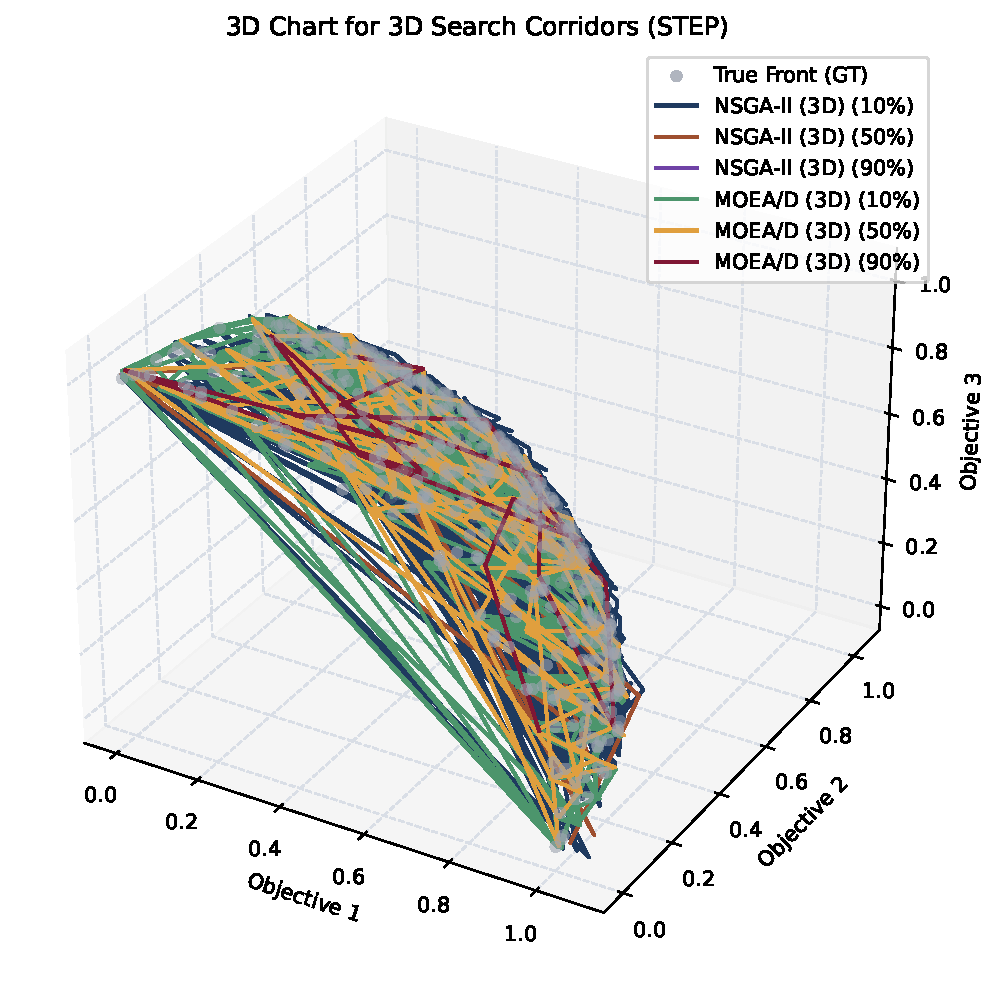
\includegraphics[width=\linewidth,height=.54\textheight,keepaspectratio]{figures/example_16_01_bands.pdf}
\end{column}
\end{columns}
\vspace{.02cm}\textbf{Leitura:} as superfícies e os degraus mostram \emph{onde} e \emph{com que frequência} cada algoritmo atinge diferentes regiões; o número de soluções não dominadas não descreve isso sozinho.
\end{frame}

\begin{frame}[fragile]{Exemplo 12 — A mesma pergunta em duas dimensões}
\begin{columns}[T,onlytextwidth]
\begin{column}{.63\textwidth}
\centering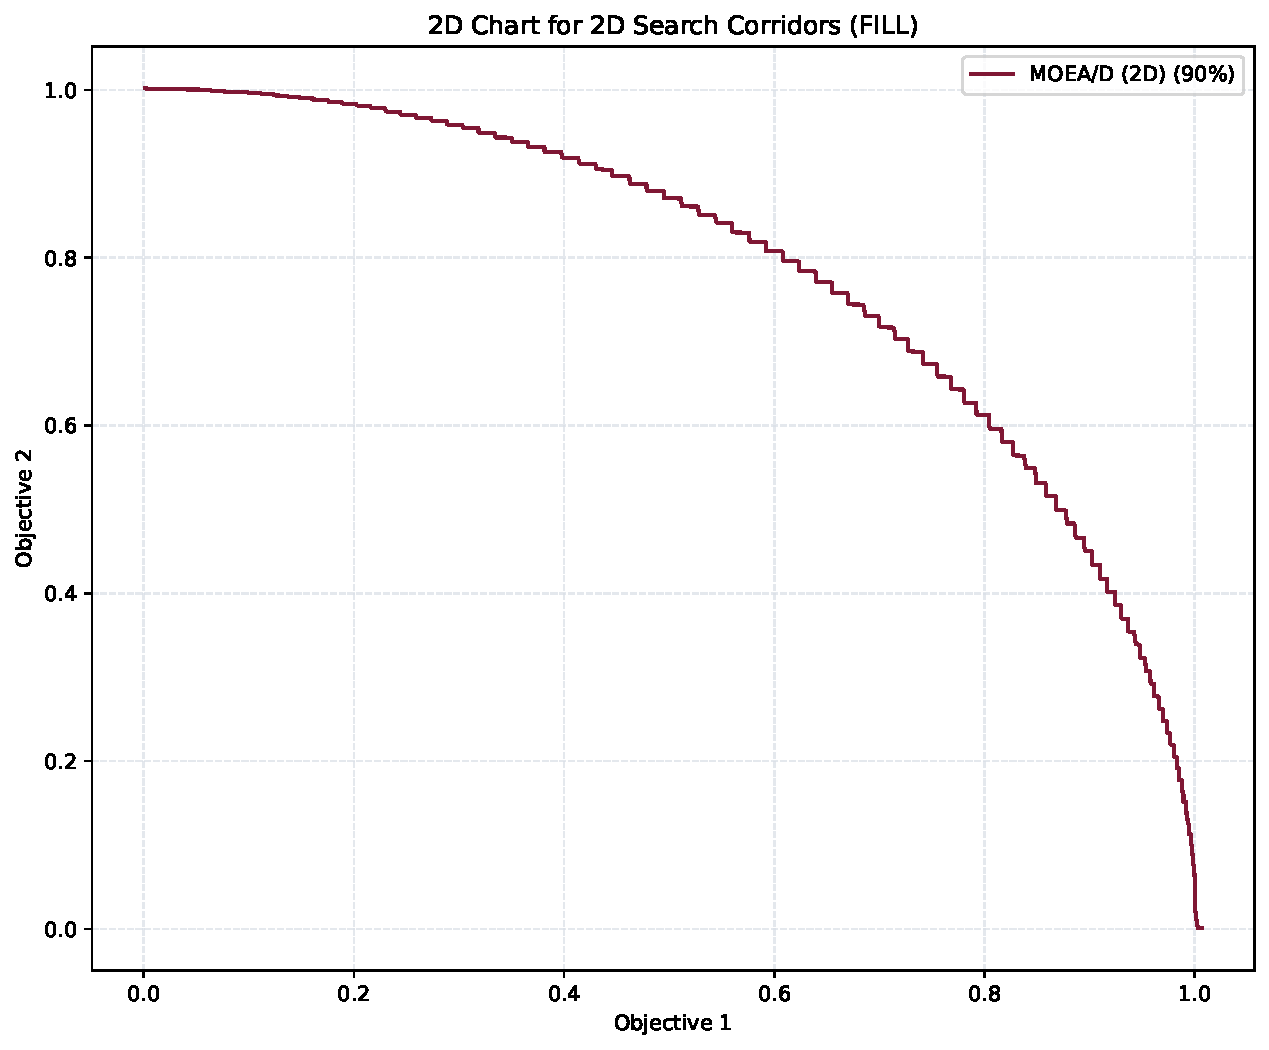
\includegraphics[width=\linewidth,height=.60\textheight,keepaspectratio]{figures/example_16_03_bands.pdf}
\end{column}
\begin{column}{.35\textwidth}
\begin{lstlisting}[style=python,basicstyle=\ttfamily\fontsize{7.2}{9}\selectfont]
mb.view.bands(
    exp1_2D, exp2_2D,
    levels=[0.1,0.5,0.9],
    style='fill')
\end{lstlisting}
\textbf{Não dominadas na união:}
\par NSGA-II: \textbf{674}
\par MOEA/D: \textbf{370}
\end{column}
\end{columns}
\vspace{.02cm}\textbf{Intuição:} maior separação entre as curvas de atingimento corresponde a maior variabilidade entre execuções naquela região do espaço de objetivos. A representação preenchida facilita a leitura do corredor bidimensional.
\end{frame}
